\chapter{Projektmanagement}

\section{Vorgehensmodell}

Als Vorgehensmodell für die \acl{ba} wurde Scrum\cite{Scrum} verwendet.
Scrum ist ein Vorgehensmodell für agile Softwareentwicklung. 

\section{Rollen}

\subsection{Product Owner}
Der Produkt Owner legt die Produkteigenschaften fest (welche Funktionen eingebaut werden müssen) 
und priorisiert diese im Backlog. Anhand der Priorität weiss man, welche 
Funktionen im nächsten Sprint erledigt sein sollten.

\subsection{Scrum Master}
Der Scrum Master kümmert sich fortlaufend darum, dass sich das Team an den Scrum 
Prozess hält und moderiert vielmals die Daily Scrums.

\subsection{Entwicklungsteam}
Das Entwicklungsteam besteht aus allen für das Projekt tätigen Entwicklern.

\section{Artifakte}

\subsection{Product Backlog}
Im Product Backlog werden die Anforderungen an das Produkt abgelegt und 
dynamisch erweitert. Dabei liegt die Verantwortung beim Product Owner, den 
Backlog zu pflegen.

\subsection{Sprint Backlog}
Im Sprint Backlog sind alle für den aktiven Sprint zu erledigenden Aufgaben 
hinterlegt, dabei liegt die Verantwortung bei den Teammitgliedern, diesen zu 
pflegen.

\subsection{Product Increment}
Beim Product Increment handelt es sich um das Endprodukt eines Sprints, dieses muss 
der Definition of Done entsprechen und in einem nutzbaren Zustand sein.
Dadurch wird sichergestellt, dass am Ende des Sprints immer eine nutzbare Software 
oder ein anderes Ergebnis zur Verfügung steht.

\section{Sprints}
In Scrum werden Iterationen über Sprints beschrieben, diese dauern in der Regel 
2 - 3 Wochen, am Ende eines Sprints soll ein auslieferbares Ergebnis zur Verfügung 
stehen.

\section{Rollen und Verantwortlichkeiten}

%Ivan Bütler
\subsection{\ibuf}

\begin{minipage}[t]{0.25\textwidth}
	\vspace{0pt}
	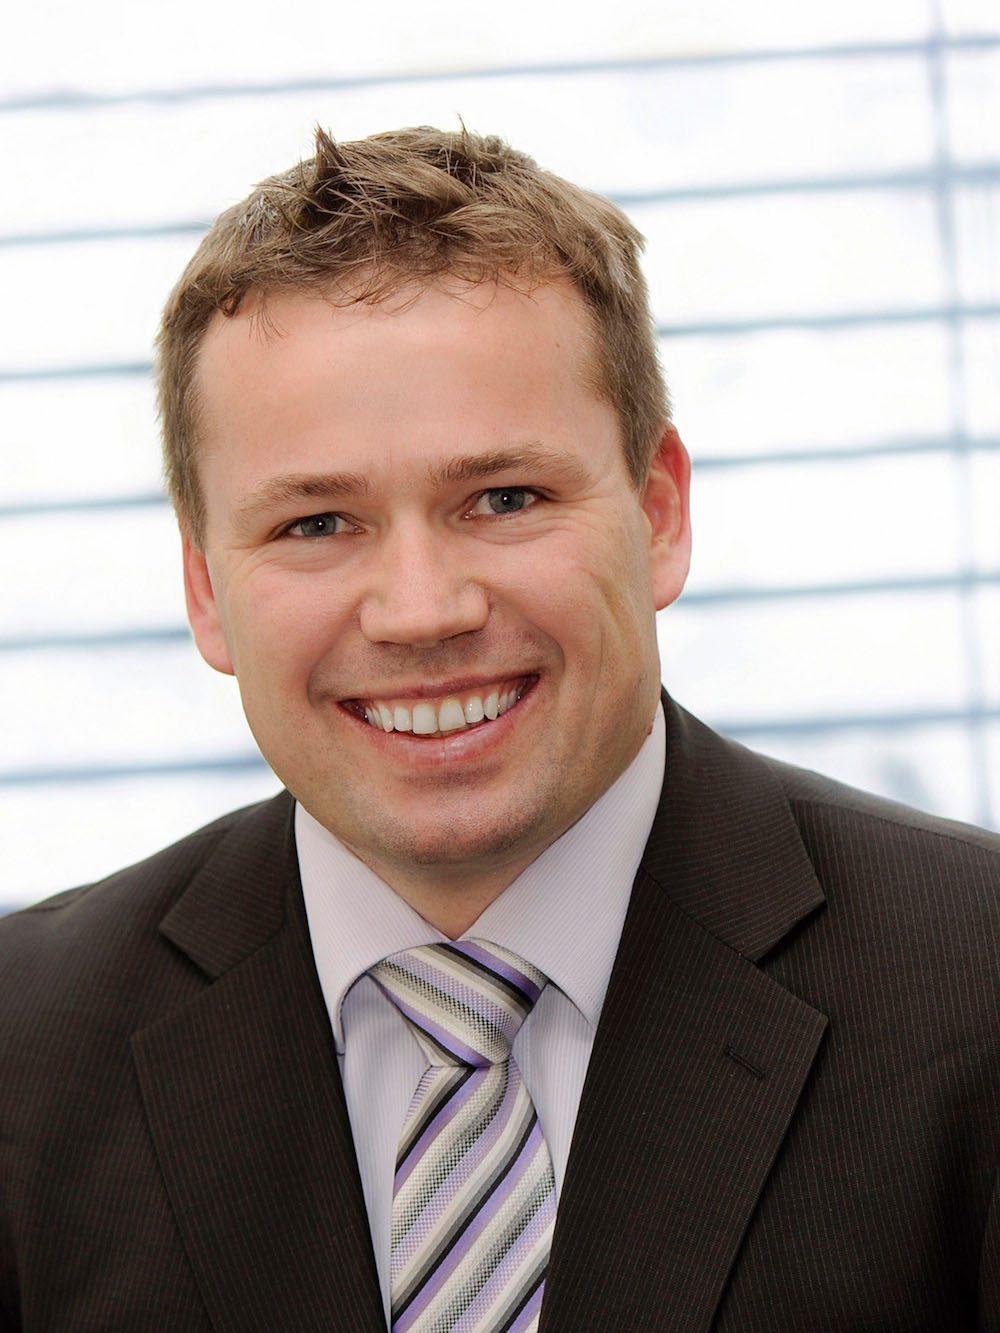
\includegraphics[width=0.8\textwidth]{img/ivan}
\end{minipage}
\begin{minipage}[t]{0.75\textwidth}
	\vspace{0pt}
	\ibu nimmt als Auftraggeber und Betreuer an dem Projekt teil (Product Owner).
\end{minipage}

%Silvan Adrian
\subsection{\sadf}

\begin{minipage}[t]{0.25\textwidth}
	\vspace{0pt}
	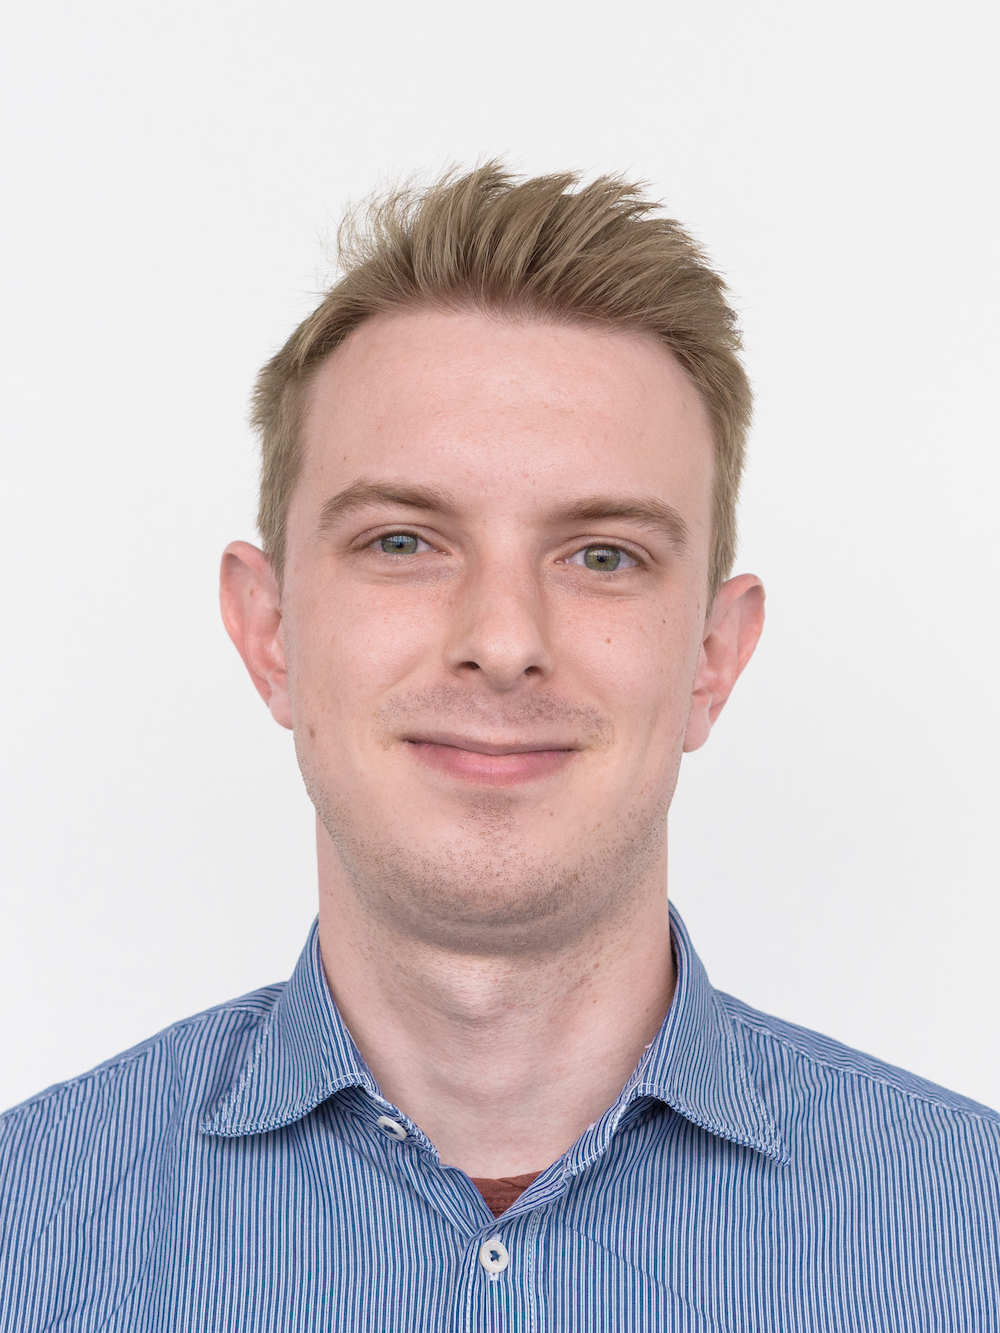
\includegraphics[width=0.8\textwidth]{img/silvan}
\end{minipage}
\begin{minipage}[t]{0.75\textwidth}
	\vspace{0pt}
	\sad, Student an der \gls{hsr}, ist Teil des Entwicklungsteams.
\end{minipage}

%Fabian Binna
\subsection{\fbif}

\begin{minipage}[t]{0.25\textwidth}
        \vspace{0pt}
	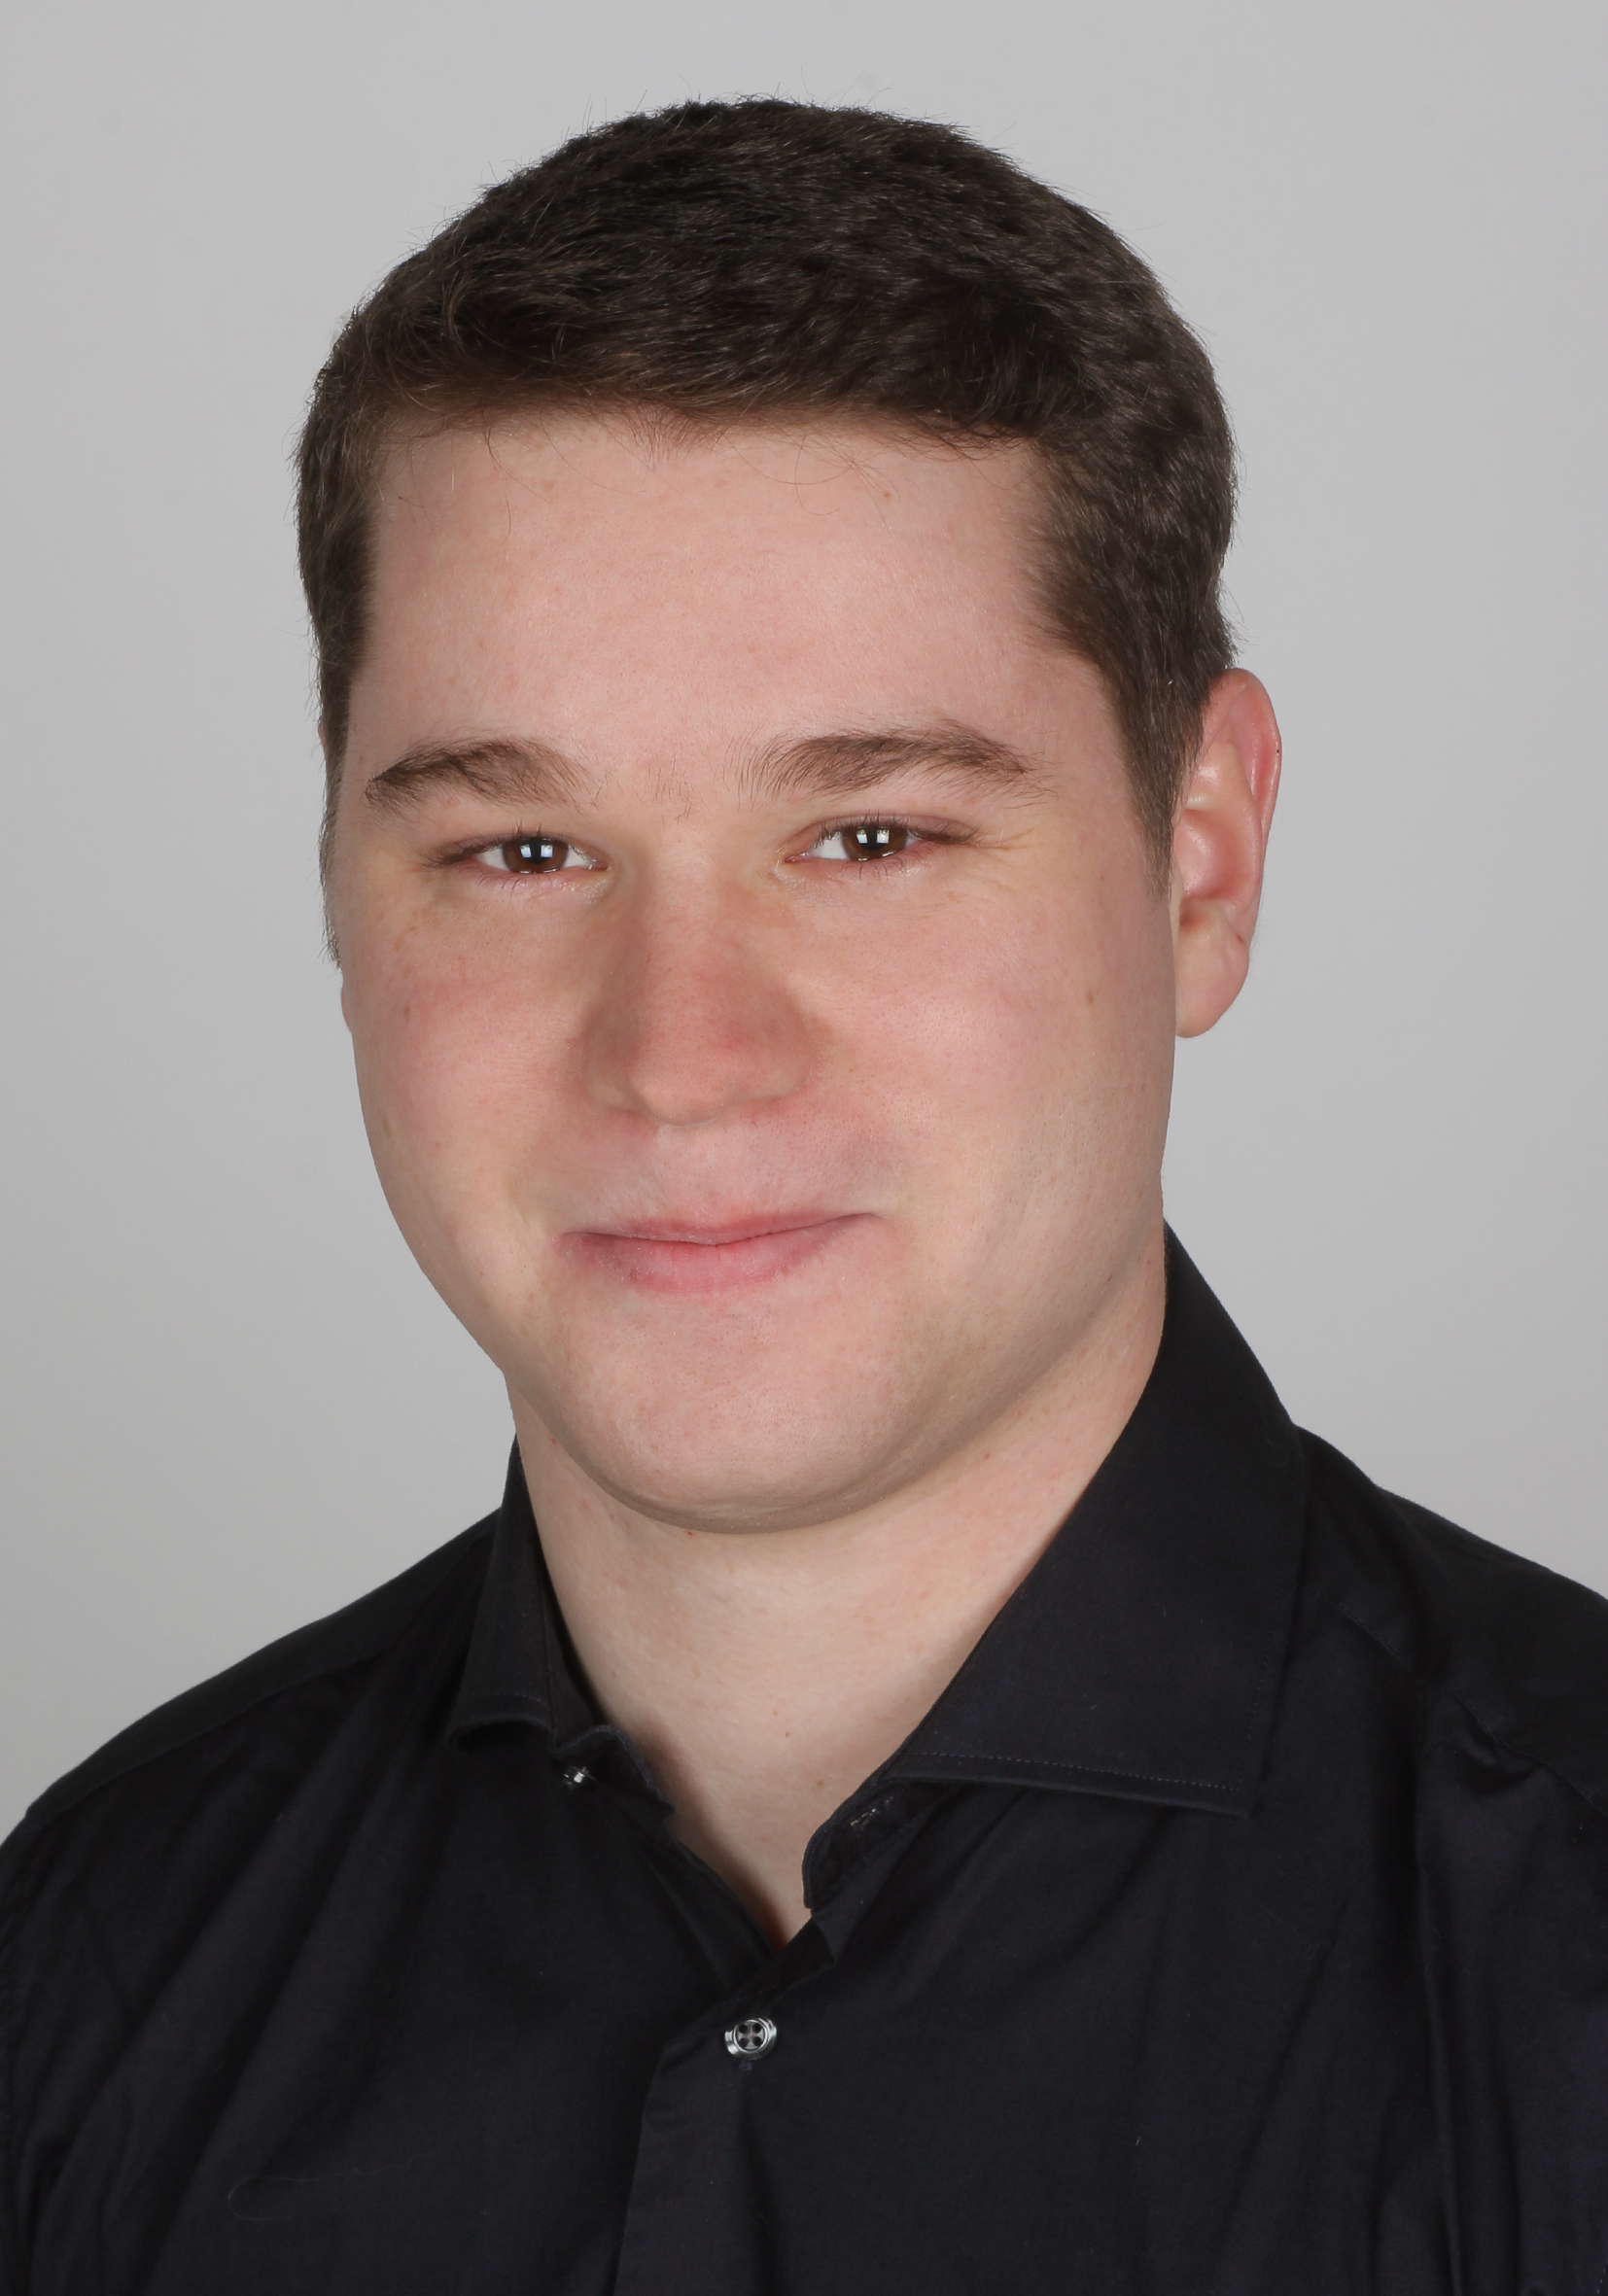
\includegraphics[width=0.8\textwidth]{img/fabian}
\end{minipage}
\begin{minipage}[t]{0.75\textwidth}
	\vspace{0pt}
	\fbi, Student an der \gls{hsr}, ist Teil des Entwicklungsteams.
\end{minipage}

\section{Risiken}
Das Risikomanagement soll bei der Planung der Sprints helfen, indem der Schaden der Risiken in die Story Points der User Stories einfliesst. Es gibt dafür keinen definierten Algorithmus, das Risikomanagement wird bei der Planung nur als Hilfe hinzugezogen. So können User Stories mit potenziellem Risiko stärker priorisiert werden.\\
Die Schadensberechnung setzt sich aus Schadenspotenzial und Eintrittswahrscheinlichkeit zusammen. Das Schadenspotenzial reicht von Eins bis Zehn. Auf eine genaue Stundenberechnung wird verzichtet.\\
Ein Risiko gilt als klein, wenn der Schaden unter Drei liegt. Bei einem Schaden über 7 ist das Risiko als hoch zu betrachten. Vor jedem Sprint wird eine neue Risikoanalyse durchgeführt, bei der die Risiken nach unten oder oben korrigiert werden. Verändert wird nur die Eintrittswahrscheinlichkeit.

\begin{landscape}
  \subsection{Initiale Risiken}
  	\begin{table}[H]		
		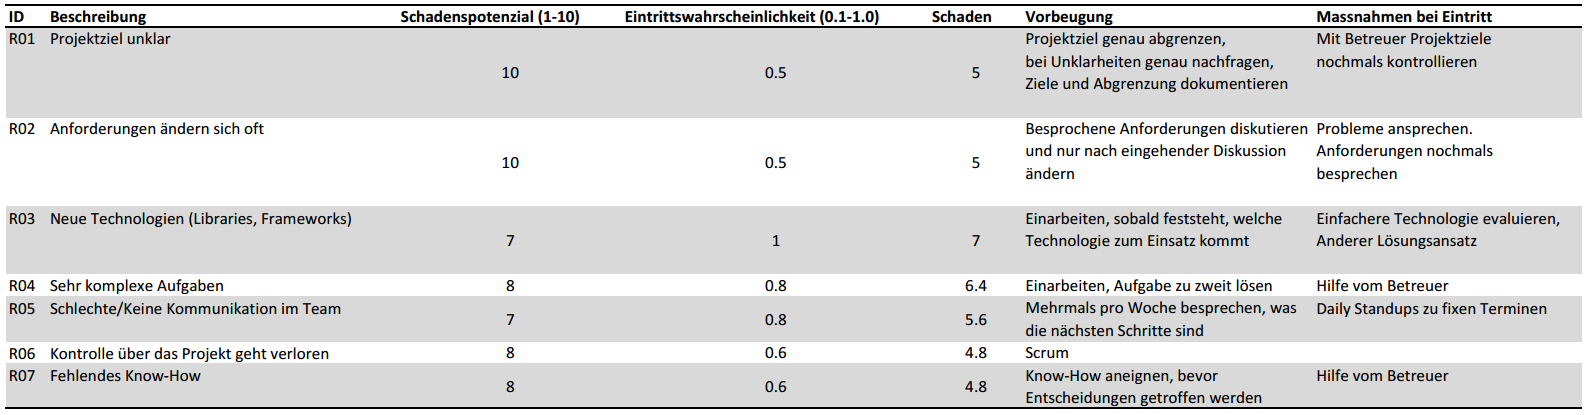
\includegraphics[width=\linewidth, keepaspectratio]{risiken/Initiales-Risikomanagement.png}
		\caption{Projektmanagement: Initiale Risiken}
	\end{table}
  	\vfill
\end{landscape}
  	   
\begin{landscape}  	   
  \subsection{Risiken Sprint 1}
  	\begin{table}[H]		
  	    \centering	
		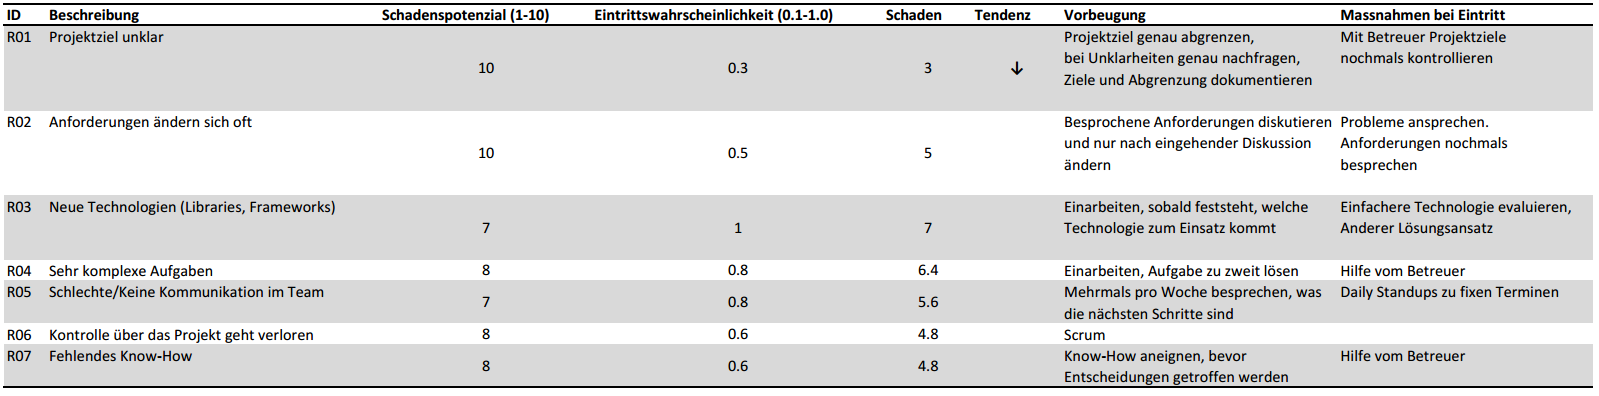
\includegraphics[width=\linewidth,keepaspectratio]{risiken/Risiken-Sprint-1.png}
		\caption{Projektmanagement: Risiken Sprint 1}
	\end{table}
	
	\subsubsection{Beschreibung}
	\begin{itemize}
		\item R01: Durch die Gespräche während den Sitzungen mit Herrn Bütler und aufgrund der schriftlichen Aufgabenstellung sind die Projektziele klarer geworden.
	\end{itemize}
	
\end{landscape}

\begin{landscape} 
    \subsection{Risiken Sprint 2}
  	\begin{table}[H]		
  	       \centering	
		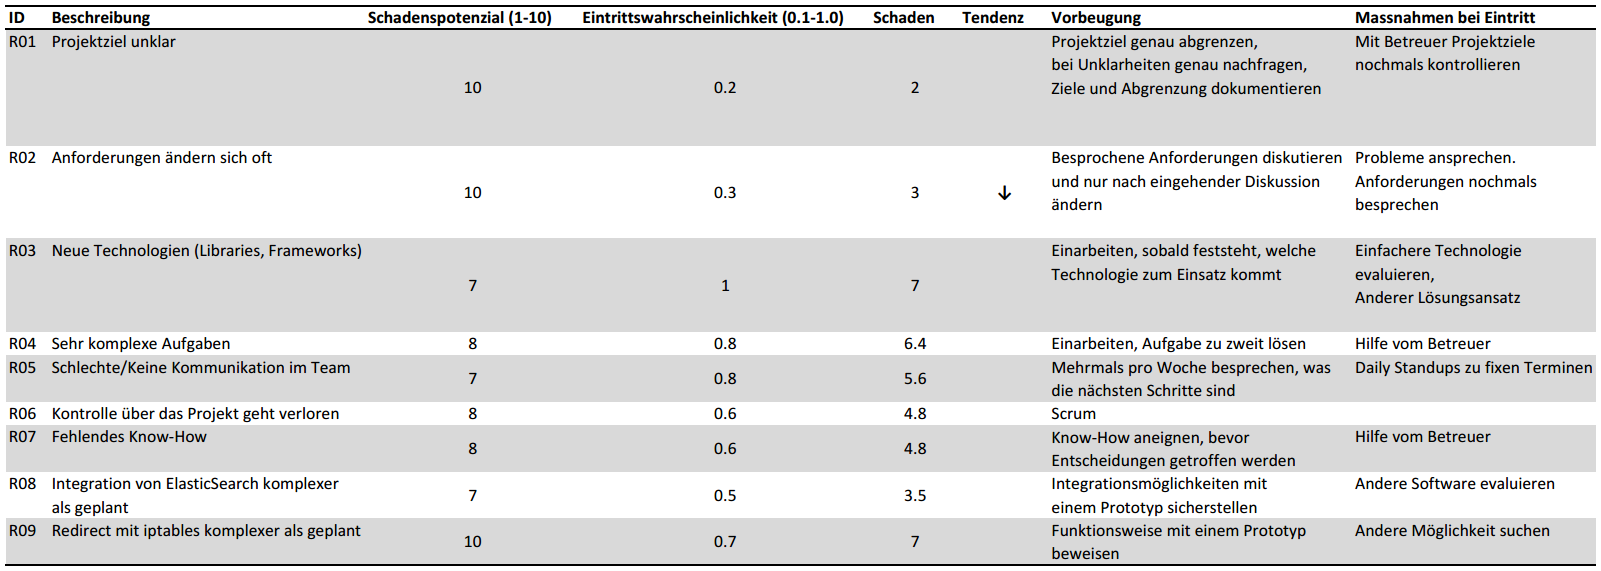
\includegraphics[width=\linewidth,keepaspectratio]{risiken/Risiken-Sprint-2.png}
		\caption{Projektmanagement: Risiken Sprint 2}
	\end{table}
	
	\subsubsection{Beschreibung}
	\begin{itemize}
		\item R02: Weitere Gespräche haben gezeigt, dass zwar neue Anforderungen gestellt werden, die bestehenden ändern sich dadurch aber nicht.
		\item R08: Es wurde beschlossen, Elasticsearch als Datenbank zu verwenden, aus Unerfahrenheit mit diesem Produkt wurde dieses Risiko definiert.
		\item R09: Es wurde beschlossen, Iptables für den Redirect zu verwenden. Da noch keine Analysen gemacht wurden und es unklar ist, ob sich Iptables dafür eignen, wurde dieses Risiko definiert.
	\end{itemize}
\end{landscape}

\begin{landscape}
  \subsection{Risiken Sprint 3}
  	\begin{table}[H]		
		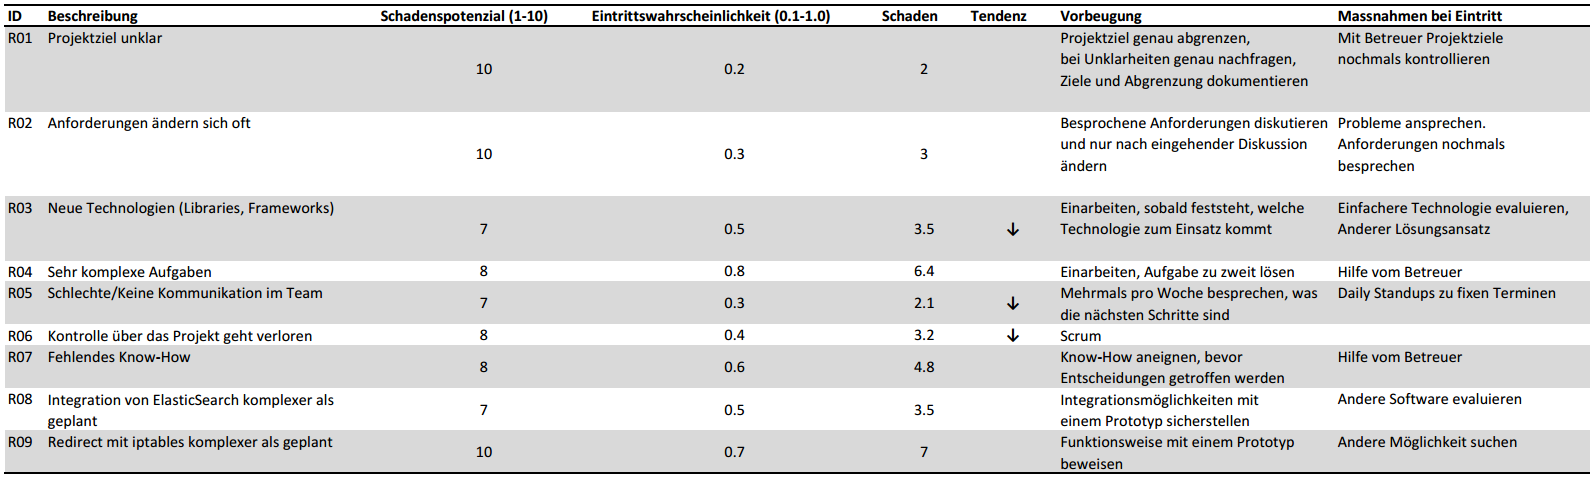
\includegraphics[width=\linewidth, keepaspectratio]{risiken/Risiken-Sprint-3.png}
		\caption{Projektmanagement: Risiken Sprint 3}
	\end{table}

	\subsubsection{Beschreibung}
	\begin{itemize}
		\item R03: Der Projektverlauf hat gezeigt, dass wir das Wissen über die neuen Technologien erlernen konnten.
		\item R05: Aufgrund von Kommunikationsproblemen wurde ein fixes wöchentliches Meeting definiert, das die Kommunikation verbessert hat.
		\item R06: Die Retrospektiven haben gezeigt, dass alle Teilnehmer das Projekt im Überblick behalten konnten.
	\end{itemize}		
	
  	\vfill
\end{landscape}

\begin{landscape}
  \subsection{Risiken Sprint 4}
  	\begin{table}[H]		
		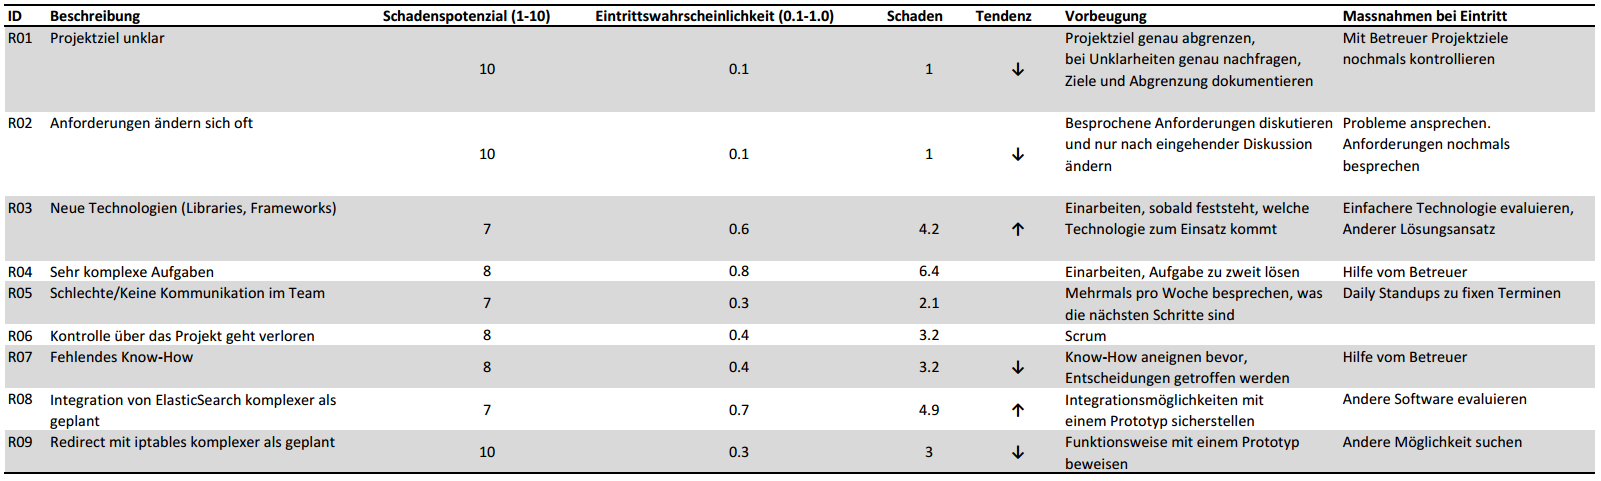
\includegraphics[width=\linewidth, keepaspectratio]{risiken/Risiken-Sprint-4.png}
		\caption{Projektmanagement: Risiken Sprint 4}
	\end{table}
	
	\subsubsection{Beschreibung}
	\begin{itemize}
		\item R01 und R02: Das Projekt nähert sich dem Ende, deshalb werden keine weiteren Anforderungen erwartet.
		\item R07 und R09: Die Analysen sind grösstenteils abgeschlossen, deshalb werden keine weiteren Probleme erwartet.
		\item R03 und R08: Das Entschlüsseln der Payloads soll neu Logstash übernehmen. Es sind wenig Erfahrungen über Logstash vorhanden.
	\end{itemize}		
	
  	\vfill
\end{landscape}

\section{Entwicklungsumgebung und Infrastruktur}

\subsection{\gls{ide}}
Als \gls{ide} wurde während des Projekts Atom, Webstorm, pyCharm und RubyMine verwendet.

\subsection{Software-Configuration-Management}
Als \gls{scm} wurde eine eigene GitLab Organisation mit verschiedenen Gitlab 
Repositories verwendet.


\subsection{Projektmanagement}
Als Projektmanagement Tool wurde Jira von Atlassian als Cloud Hosted Software verwendet, um  
nicht viel Zeit mit der Server Konfiguration zu vergeuden.
Jira bietet alle möglichen Tools und Funktionen, um ein agiles Softwareprojekt 
zu planen und durchzuführen.

\subsection{Kommunikation}
Bei der Durchführung  der Bachelorarbeit wurde auf Slack gesetzt, was einen 
einfachen Austausch unter den Teammitgliedern ermöglicht, ebenfalls gibt es Integrationen zu 
Gitlab und anderen Services, womit man immer über die neusten Änderungen benachrichtigt 
wird.


\section{Qualitätsmanagement}

\subsection{Dokumentation}
Die Dokumentation befindet sich auf einem privaten Gitlab Repository. 
Versionen werden mit Git Tags versehen. Bei grösseren Dokumentationsarbeiten muss ein Pull Request gemacht werden. Die Dokumentation wird in \LaTeX geschrieben und mit Gitlab-CI kompiliert. Sitzungsprotokolle sind über die Gitlab Page (\href{https://hsr-ba-hs16-cc.gitlab.io/ba-doc/}{https://hsr-ba-hs16-cc.gitlab.io/ba-doc/}) im PDF Format einsehbar. 

\subsection{Projektmanagement Tool}
Als Projektmanagement Tool wird Jira verwendet.\\
\href{https://cc-proxy.atlassian.net/projects/CC/summary}{https://cc-proxy.atlassian.net/projects/CC/summary}

\subsection{Metriken}
Metriken waren nicht nötig, da während dem Projekt relativ wenig Code geschrieben wurde.

\subsection{Testing}
\subsubsection{Systemtest}
Die Verifizierung der Systemtests richtet sich nach den Anforderungen und Use Cases. Die Systemtests müssen manuell durchgeführt werden.

\subsection{Definition of Done}

\subsubsection{Review}
Der Reviewprozess garantiert die Qualität der Arbeit. Es wird immer auf einem Feature Branch gearbeitet. Im Pull Request wird ein aussagekräftiger Title verwendet. In der Beschreibung des Pull Requests befindet sich eine aussagekräftige Beschreibung. Nachdem ein anderes Teammitglied die Arbeit kontrolliert hat, kann der Pull Request als ''OK'' markiert werden. Der Feature Branch wird nach einem ''OK'' vom Entwickler selbst mit dem Master Branch zusammengeführt.

\begin{figure}[H]
	\centering
	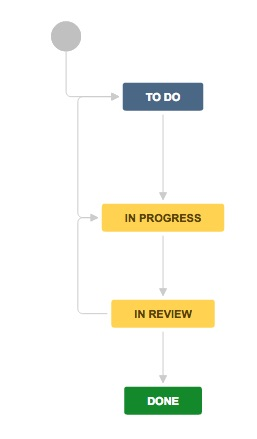
\includegraphics[scale=0.8]{img/review-workflow.jpg}
	\caption{Projektmanagement: Review Workflow}
	\label{fig:review_workflow}
\end{figure}

\subsubsection{Softwaredokumentation}
\begin{itemize}
	\item "Getting Started" beinhaltet folgende Informationen: Quick Start um Applikation aufzusetzen
	\item Installationsanleitung
	\item Benutzeranleitung
	\item Neuer \gls{cc} Workflow
\end{itemize}

\subsubsection{Testing}
Das Entwicklerteam ist verantwortlich für den zuverlässigen Betrieb der Anwendung.

\subsection{Deployment}
Der Masterbranch ist Produktion und enthält alle neuen Features. Die Demo wird auf dem Masterbranch vorgenommen.

\subimport{stories/}{stories.tex}

\subimport{sprints/}{sprints.tex}
